% *****************************************************************************
%
%        FASThesis Manual
%        (FASThesis Class File Documentation)
%
%        Faculty of Applied Sciences
%        University of West Bohemia
%
%        Manual & Explanatory Document
%        Copyright (c) 2022-2023 Kamil Ekštein, Dept. of Computer Science
%        and Engineering, Faculty of Applied Sciences, UWB
%
%        Version:  0.7
%		 Encoding: UTF-8
%		 TeXer:    pdflatex
%
%        Last modification on 28-Feb-2023 by KE
%
% *****************************************************************************

% _____________________________________________________________________________
%
%
%	     DOCUMENT HEADER
%
% _____________________________________________________________________________
%
\documentclass[czech, bc, kiv, he, iso690numb]{fasthesis}
\title{\texttt {}Vývoj Javascript knihovny pro embedování vizualizací skrze Emplifi Public API}
\author{Milan}{Janoch}{}{}
\supervisor{Doc. Ing. Dalibor Fiala, Ph.D.}
%\supervisor{Ing. Tomáš Marný}
\assignment{zadanibp.pdf}
\signdate{15}{12}{2023}{V Plzni}% << the longest local name in the Czech Rep.

\addbibresource{bp.bib}% << the file with the bibliographical database to be used throughout the text

% _____________________________________________________________________________
%
%
%	     DOCUMENT FRONTMATTER TEXTS
%
% _____________________________________________________________________________
%
\abstract{Tato bakalářská práce se zaměřuje na vývoj specializované JavaScript knihovny s cílem umožnit snadné embedování vizualizací do aplikací třetích stran. Hlavními cíli práce jsou návrh a implementace knihovny, navržení rozhraní pro efektivní komunikaci s Public API firmy Emplifi a zajištění bezpečného přístupu k datům pomocí OAuth 2 protokolu. V teoretické části práce je diskutována problematika spojená s embedováním vizualizací do externích aplikací, bezpečný přístup k datům třetích stran a jsou analyzována již existující řešení. Praktická část se zaměřuje na návrh a implementaci JavaScript knihovny, popisuje navržení rozhraní pro efektivní komunikaci s API a zabývá se implementací bezpečného přístupu k datům v souladu se standardem OAuth 2.
}
% *** English abstract ***
{This bachelor thesis focuses on the development of a specialized JavaScript library to enable easy embedding of visualizations into third-party applications. The main goals of the thesis are to design and implement the library, design an interface to communicate efficiently with Emplifi's Public API and provide secure data access using the OAuth 2 protocol. The theoretical part of the thesis discusses the issues related to embedding visualizations in external applications, secure access to third-party data and analyzes existing solutions. The practical part focuses on the design and implementation of a JavaScript library, describes the design of interfaces for efficient communication with APIs and deals with the implementation of secure data access in accordance with the OAuth 2 standard.}
\keywords{OAuth 2.0, embedování, Emplifi Public API, token, JavaScript}
% _____________________________________________________________________________
%
%        ACKNOWLEDGEMENT
% _____________________________________________________________________________
%
\acknowledgement{Na tomto místě bych rád poděkoval všem, kteří přispěli k úspěšnému dokončení této bakalářské práce.
Velké díky patří především

Bc. Ondřejovi Altmanovi za trpělivost, cenné rady a vstřícnost při navrhování a implementaci praktické části 

Ing. Michalovi Kacerovskému za poskytování připomínek v rámci detailní revize kódu, která významně přispěla k vylepšení čitelnosti a efektivity kódu

Monice Opltové za důkladné a pečlivé otestování implementované praktické části

Doc. Ing. Daliborovi Fialovi, Ph.D. za jeho podporu a ochotu při tvorbě teoretické části

a také rodině za podporu během celého studia.
}
% _____________________________________________________________________________
%
%
%	     DOCUMENT TEXT BEGINNING
%
% _____________________________________________________________________________
%
\begin{document}
\frontpages[tm] % or notm if the `trademark' declaration is not needed
\tableofcontents
% 
% -x---- ADDITIONAL COLOUR DEFINITIONS ----------------------------------------
%
\makeatletter%
\ifx\FASThesis@style\c@fullcolor%
	\definecolor{fascolor}{cmyk}{0.06, 0.27, 1.0, 0.12}%
	\definecolor{fascolordk}{cmyk}{0.05, 0.28, 1.0, 0.24}%
\else%
	\definecolor{fascolor}{cmyk}{0, 0, 0, 0.6}%
	\definecolor{fascolordk}{cmyk}{0, 0, 0, 0.75}%
\fi%
\makeatother%
\lstdefinestyle{plainsrc}{
	backgroundcolor=\color{fascolor!10},
	basicstyle=\ttzfamily\footnotesize,
	numberstyle=\tiny\color{fascolordk},
	numbers=left,
	numbersep=5pt,
	keepspaces=true,
	tabsize=2,
	extendedchars=true,
	literate={á}{{\'a}}1 {č}{{\v{c}}}1 {ď}{{\v{d}}}1 {é}{{\'e}}1 {ě}{{\v{e}}}1 {è}{{\`{e}}}1 {í}{{\'{\i}}}1 {ľ}{{\v{l}}}1 {ň}{{\v{n}}}1 {ó}{{\'o}}1 {ŕ}{{\'r}}1 {ř}{{\v{r}}}1 {š}{{\v{s}}}1 {ť}{{\v{t}}}1 {ú}{{\'u}}1 {ů}{{\r{u}}}1 {ý}{{\'y}}1 {ž}{{\v{z}}}1
	{Á}{{\'A}}1 {Č}{{\v{C}}}1 {Ď}{{\v{D}}}1 {É}{{\'E}}1 {Ě}{{\v{E}}}1 {È}{{\`{E}}}1 {Í}{{\'I}}1 {Ľ}{{\v{L}}}1 {Ň}{{\v{N}}}1 {Ó}{{\'O}}1 {Ŕ}{{\'R}}1 {Ř}{{\v{R}}}1 {Š}{{\v{Š}}}1 {Ť}{{\v{T}}}1 {Ú}{{\'U}}1 {Ů}{{\r{U}}}1 {Ý}{{\'Y}}1 {Ž}{{\v{Z}}}1
}

% Nastavení vzhledu pro JSON
\definecolor{json_keyword}{rgb}{0.13,0.55,0.13}
\definecolor{json_string}{rgb}{0.31,0.60,0.02}

\lstdefinelanguage{json}{
    basicstyle=\normalfont\ttfamily,
    numbers=left,
    numberstyle=\tiny,
    stepnumber=1,
    numbersep=8pt,
    showstringspaces=false,
    breaklines=true,
    frame=lines,
    backgroundcolor=\color{gray!10},
    literate=
     *
      {:}{{{\color{blue}{:}}}}{1}
      {,}{{{\color{blue}{,}}}}{1}
      {\{}{{{\color{blue}{\{}}}}{1}
      {\}}{{{\color{blue}{\}}}}}{1}
      {[}{{{\color{blue}{[}}}}{1}
      {]}{{{\color{blue}{]}}}}{1},
}
% _____________________________________________________________________________
%
%
%        CHAPTER
%
% _____________________________________________________________________________
%
\chapter{Úvod}
V současné době internetu tvoří data významnou a důležitou součást každodenního života. Problematikou dat je nejen je efektivní ukládání, 
ale také rychlé a efektivní interpretování. 
Vizualizace dat není pouhým trendem, ale stala se klíčovým nástrojem v mnoha odvětvích. Od oblasti logistiky, kde pomáha monitorovat a řídit tok zásob a logistické operace, až po oblast sociálního marketingu, kde je využívána na k personalizovaným reklamám či sledování aktivit zákazníků. 
Pro snadné integrování vizualizací do aplikací třetích stran se využívá koncept embedded analytics – ten umožňuje uživatelům rychlý a efektivní přístup k datům bez potřeby přecházet mezi různými aplikacemi. 

Cílem této práce, zadanou společností Emplifi, která se specializuje na sociální marketing, je vytvořit praktickou knihovnu umožňující embedování analytických grafů do aplikací třetích stran. 
Velký důraz bude kladen na bezpečný přístup k datům skrze OAuth 2 protokol, který je klíčovým prvkem Emplifi Public API. Součástí bude také administrační rozhraní, jenž umožní snadné generování a obnovování OAuth 2 tokenu, a podrobná uživatelská dokumentace, která bude obsahovat veškeré informace k nastavení a používání knihovny či uživatelského rozhraní.

V rámci teoretické části bude podrobně diskutována problematika spojená s embedováním. Analyzovat se bude princip, výhody a nevýhody bezpečnostního protokolu OAuth 2 a již existující řešení embedded analytics.

Tímto způsobem práce nespojuje pouze technologickou inovaci s nutností bezpečnosti dat, ale také reaguje na aktuální potřeby v odvětví sociálního marketingu a digitálního prostoru.
% _____________________________________________________________________________
%
%
%        CHAPTER Embbedded analytics a zabezpečení
%
% _____________________________________________________________________________
%
\chapter{Embedded analytics a zabezpečení}
V této kapitole se zmíníme o principu embedded analytics, zabezpečení dat pomocí OAuth 2 tokenu a již existujících řešeních.

%
%   Podkapitola princip
%
\section{Princip}
Embedded analytics transformuje data do grafů a dashboardů \cite{goodDataEmbedded}. Dashboard je souhrn informací a nástrojů, který umožňuje rychle a jednoduše zobrazovat důležité metriky (např. počet komentářů pod příspěvkem) \cite{coJeDashboard}.
Emplifi dashboardy umožňují definovat, vytvářet a vizualizovat aktivity uživatelů na sociálních sítí \cite{emplifiDashboard}, což umožňuje komplexní pohled na interakci s obsahem.

\begin{figure}
	\centering
	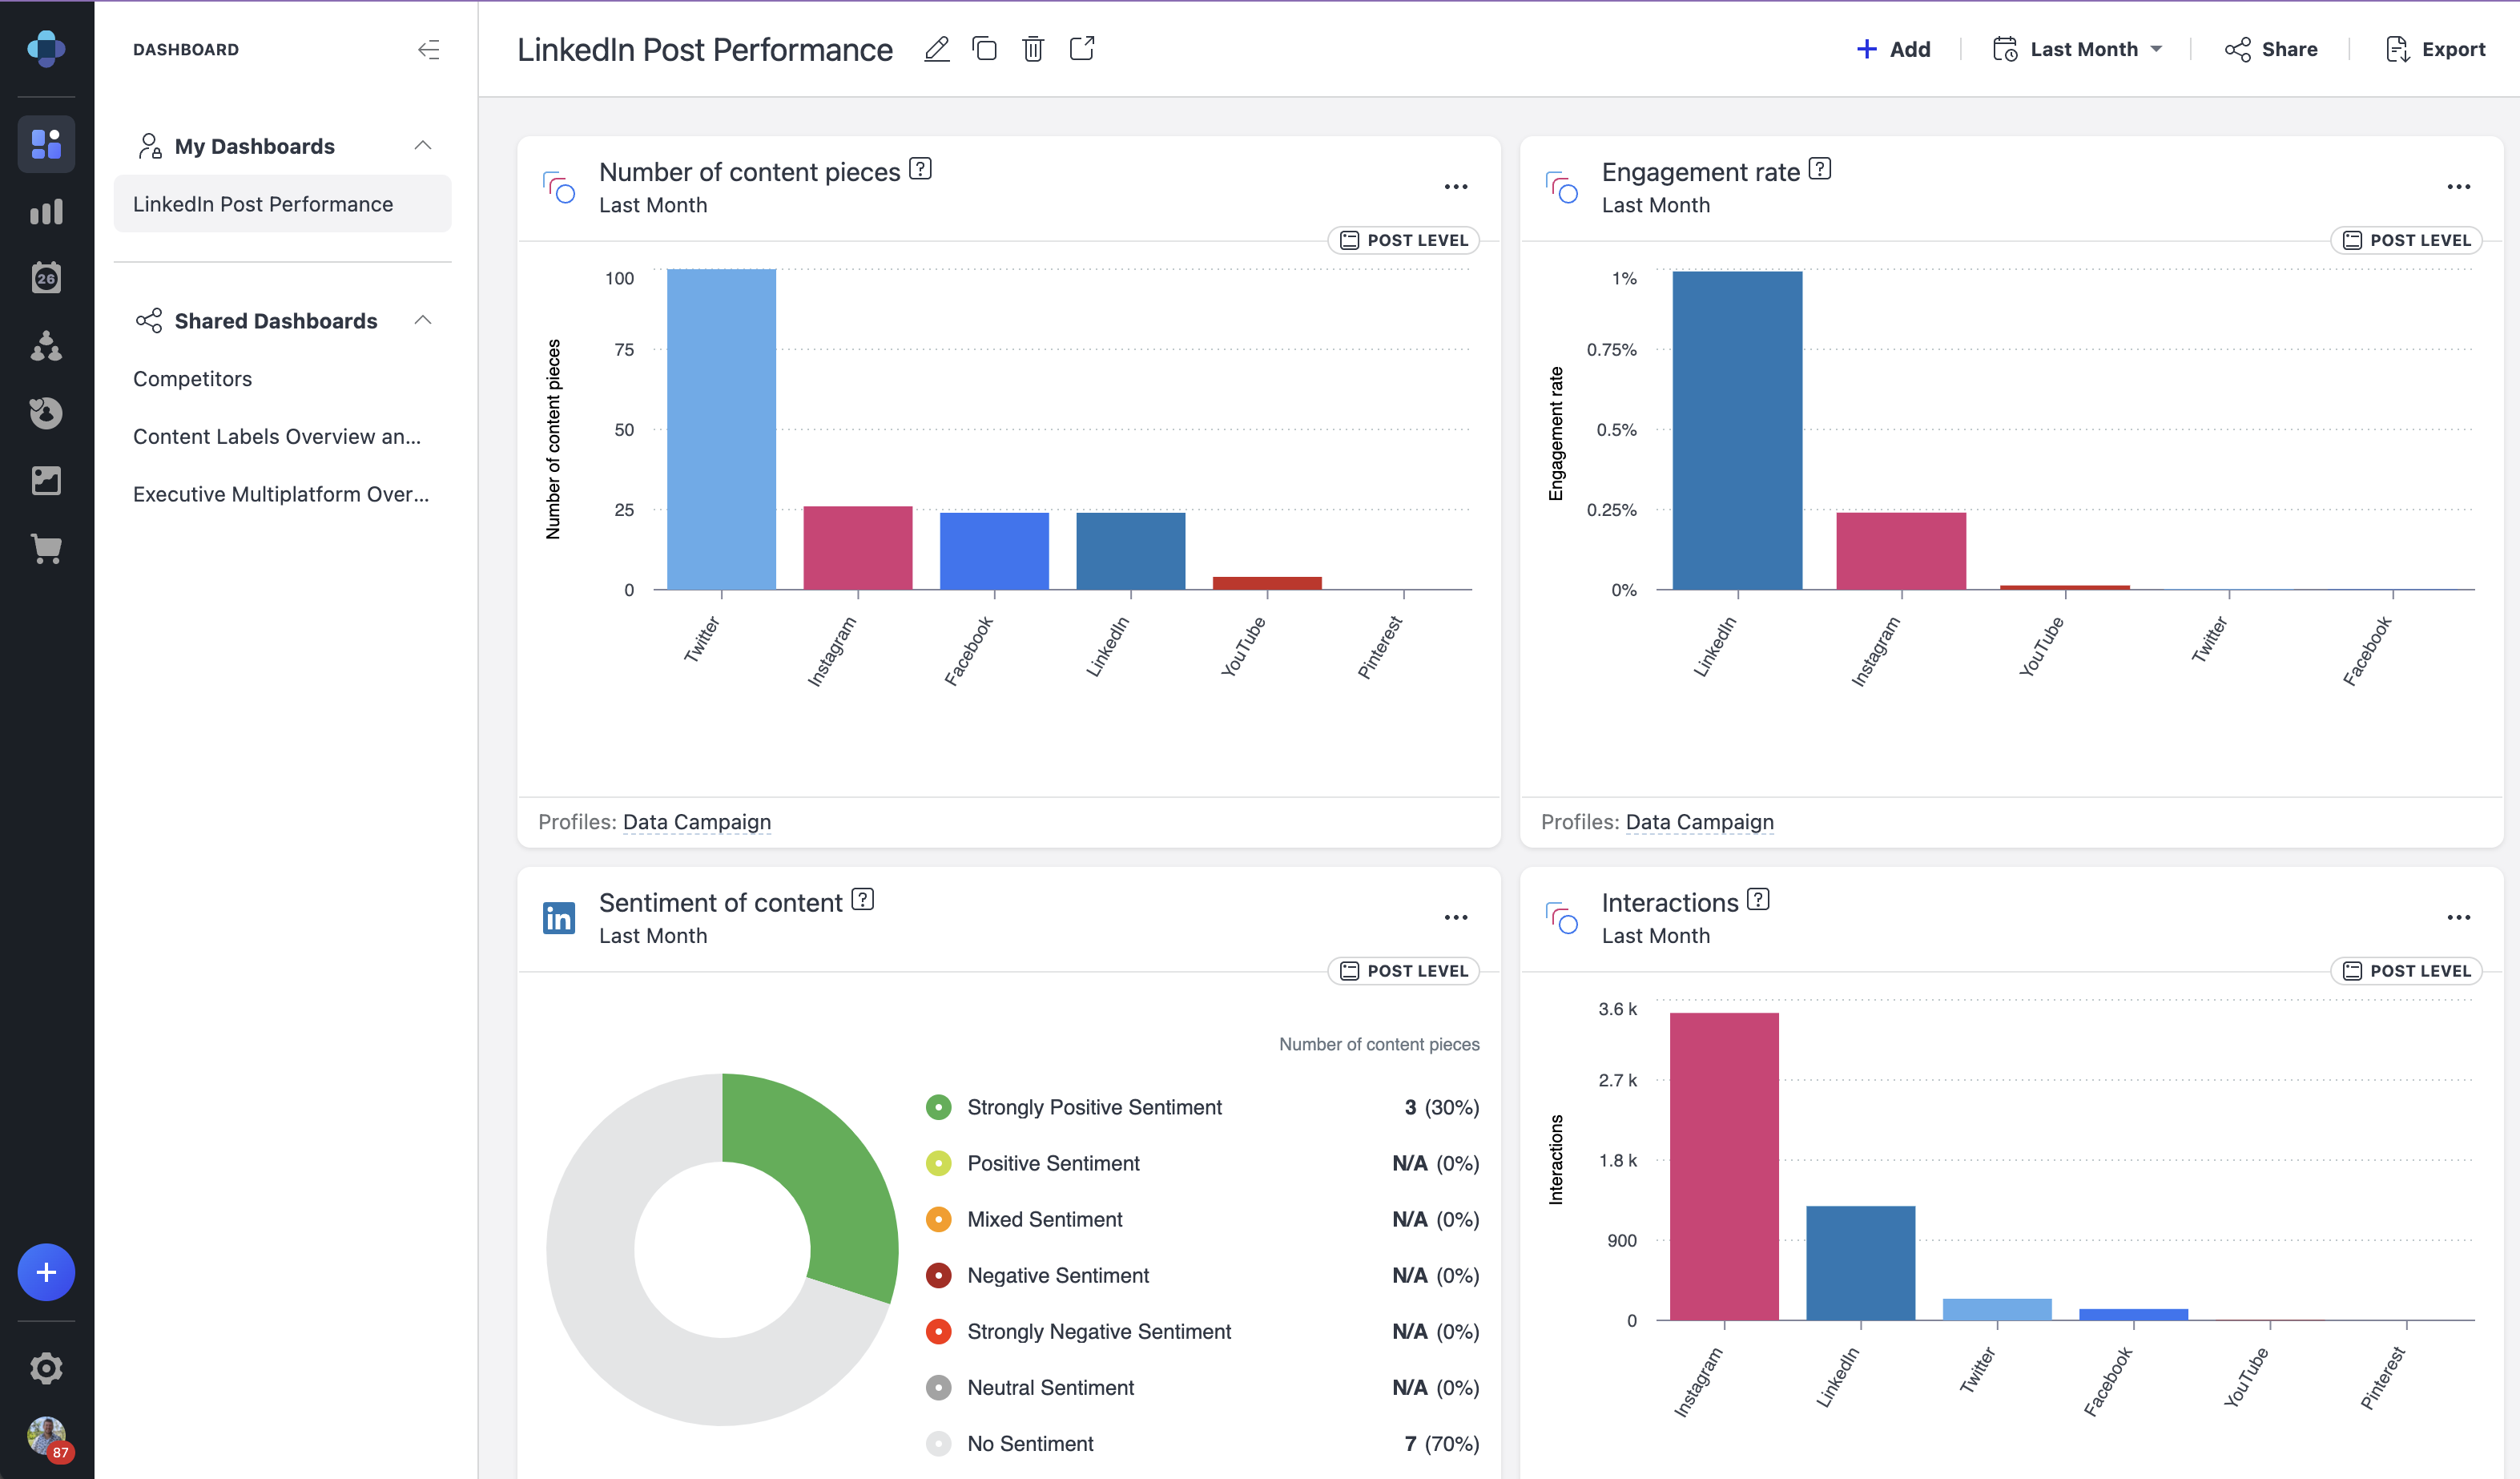
\includegraphics[width=1\textwidth]{pictures/emplifi-dashboard-example.png}
	\caption{Ukázka dashboardu v produktu firmy Emplifi}
	\label{fig:emplifiDashUkazka}
\end{figure}

Na obrázku \ref{fig:emplifiDashUkazka} vidíme příklad dashboardu - skládá se z několika grafů, obvykle nazývané jako widgety \cite{emplifiDashboard}, jejichž obsah lze modifikovat pomocí přepínačů v liště. Obsah může být modifikován v časovém období (posledních 30 dní, poslední rok, konkrétní časový rozsah, ...), ale lze jej modifikovat také na základě metrik jako je např. sociální síť (Facebook, Instragram, LinkedIn), druh interakcí (komentáře, liky, sdílení) apod.\footnote{Widgety nemusí být obecně pouze vizualizace, může se jednat také o ovládací prvky (např. výběrové seznamy, check boxy, textfieldy, apod.). Tato možnost se využívá zejména ve vývojářských dashboardech pro rychlejší tvorbu vizualizací. V samotném produktu firmy se ale používá kvůli uživatelské přívětivosti pouze pro vizualizace \cite{emplifiDashboard}. 
}

Embedded analytics se nechová a nevypadá jako samostatná aplikace, ale je integrován do jiného softwaru nebo webového portálu. Koncoví uživatelé často ani nepoznají, že se jedná
integrovanou analytiku a vnímají software s touto integrovanou analytikou jako jeden nástroj \cite{goodDataEmbedded}. To umožňuje softwarovým společnostem získat a plně
integrovat analytickou platformu s jejich vlastním SaaS produktem bez nutnosti velkých investic do vývoje vlastního řešení. 

SaaS (Software as a Service) je licenční model, v němž přístup je poskytován na základě předplatného, přičemž software je umístěn na externích serverech, nikoli na firemních serverech \cite{saasDefinition}.
K těmto službám se běžně přistupuje prostřednictvím webového prohlížeče s přihlašovacím jménem a heslem. Výhodou je, že místo toho, aby mělo každé zařízení ve firmě nainstalované
tento program, stačí se do programu přihlásit přes internet. Pro firmu to znamená úsporu financí, jelikož nemusí investovat do nového hardwaru, na němž by dané programy běžely. 
Nevýhodou SaaS je bezpečnost dat a rychlost jejich doručování. Protože jsou data umístěna na externích serverech, je třeba zajistit rychlé a spolehlivé internetové připojení a vyloučit
přístup neoprávněných uživatelů.

Existuje hned několik způsobů, jak data embedovat. Mezi nejpopulárnější a nejrozšířenější způsoby patří HTML iframe, webová komponenta či React SDK s voláním API \cite{goodDataEmbedded}. 

Nejjednodušší a nejrychlejší metodou embedování je využití použití iframu \cite{goodDataEmbedded}. Iframe (Inline frame) je HTML prvek, který umožňuje načíst HTML stránku uvnitř dokumentu \cite{iFrameAdv}. Používá se pro vložení určitého obsahu z jednoho zdroje do druhého. To se poté jeví jako nové okno v dané stránce, jedná se ovšem o embedovaný iframe. Tuto možnost embedování využívají např. Google Mapy nebo YouTube \cite{iFrameAdv}. Velkou výhodou je, že není třeba instalovat pro běh žádné dependence.

Pokročilejší technikou pro embedování je použití webové komponenty. Výhoda opět spočívá v tom, že není třeba instalovat závislosti pro běh. Embedování probíhá pomocí knihovny, která se naimportuje přes HTML tag \texttt{<script>}. Poté je možno embedovat vizualizace pouze prostřednictvím naimplementovaných webových komponent \cite{webComp}.

Poslední zmiňovanou možností je embedování prostřednictvím React SDK s voláním API. 

SDK (Software development kit) je označení sady nástrojů pro tvorbu softwaru \cite{SDKvsAPI}, které umožňuje vývojářům vytvářet rychleji a standartizovaně nové aplikace. API 
(Application Programming Interface) je rozhraní usnadňující komunikaci mezi dvěmi platformami. Uživatel specifikuje požadavek na data, rozhraní API provede volání na webový server, který
následně tento požadavek zpracuje a odešle odpověď na specifikované volání (může se jednat např. o data ve formátu JSON). Díky tomu se krátí vývojový cyklus (automatizace), efektivně 
se poskytují nové služby uživatelům a může zlepšit reputaci důvěryhodnost značky.

K embedování je potřeba následovat instrukce (např. nainstalování dependencí, zprovoznění backendu, apod.) a zajistit, že všechny kroky v nich obsažené budou splněny \cite{reactSDKComp}. Jedná se tedy o programátorsky náročnější metodu, ovšem výhoda spočívá ve větší flexibilitě vývojářů, kteří mohou vizualizace snadno modifikovat \cite{goodDataEmbedded}.

%
% Podkapitola zabezpečení
%
\section{Zabezpečení}
Zabezpečení API je důležitou součástí v moderním inženýrství zajišťující bezpečnou a důvěryhodnou komunikaci mezi různými aplikacemi. S rostoucím významem API pro výměnu dat mezi
systémy je nezbytné věnovat zvláštní pozornost implementaci efektivních bezpečnostních opatření. API authentication (autentizace) je řešením pro ověřování uživatelů - to umožňuje
vlastníkovi daného API ochranu před neoprávněným přístupem ze strany uživatelů, kteří nemohou ověřit svou totožnost \cite{whatIsAPI}.

Řešení autentizace jsou obvykle nastavena tak, aby zablokovala přístup do API, pokud se při volání zjistí něco nesprávného/nevalidního s uživatelem. S tím se pojí druhá bezpečnostní
složka, kterou je autorizace (authorization). Zatímco autentizace ověřuje identitu uživatele, autorizace se zabývá tím, jaké akce má daný uživatel povoleny \cite{mostUsedAuthentication}. 
Mezi nejpoužívanější metody patří HTTP authentication, API keys a OAuth 2.0. 

HTTP authentication omezuje přístup k serveru pomocí Basic HTTP schématu \cite{mozillaHTTPAuth}. Uživatel, který chce ověřit svou identitu, tak může učinit vložením hlavičky 
Authorization s bezpečnostními údaji - nejčasteji tím bývá uživatelské jméno a heslo. 

API klíč (key) je jedinečný alfanumerický řetězec, který slouží k jednoznačné identifikaci klientů/aplikací \cite{amazonAPIKey}, jenž API využívají. Narozdíl od tokenů
nejsou časově omezené - to může znamena bezpečnostní problém v případě, že při zadávání požadavku API by přenášený klíč mohl být zachycen \cite{mostUsedAuthentication}.

OAuth (Open Authorization) protokol byl vyvinut jako řešení pro udělování přístupu na předem definovanou dobu bez sdílené uživatelských jmen a hesel \cite{understandingOAuth2}. OAuth 2.0
je nejlepší volbou pro identifikaci osobních uživatelských účtů a udělování patřičných oprávnění \cite{mostUsedAuthentication}. Proces autentizace je vidět na obrázku \ref{fig:oauth2Diagram}.


\begin{figure}
	\centering
	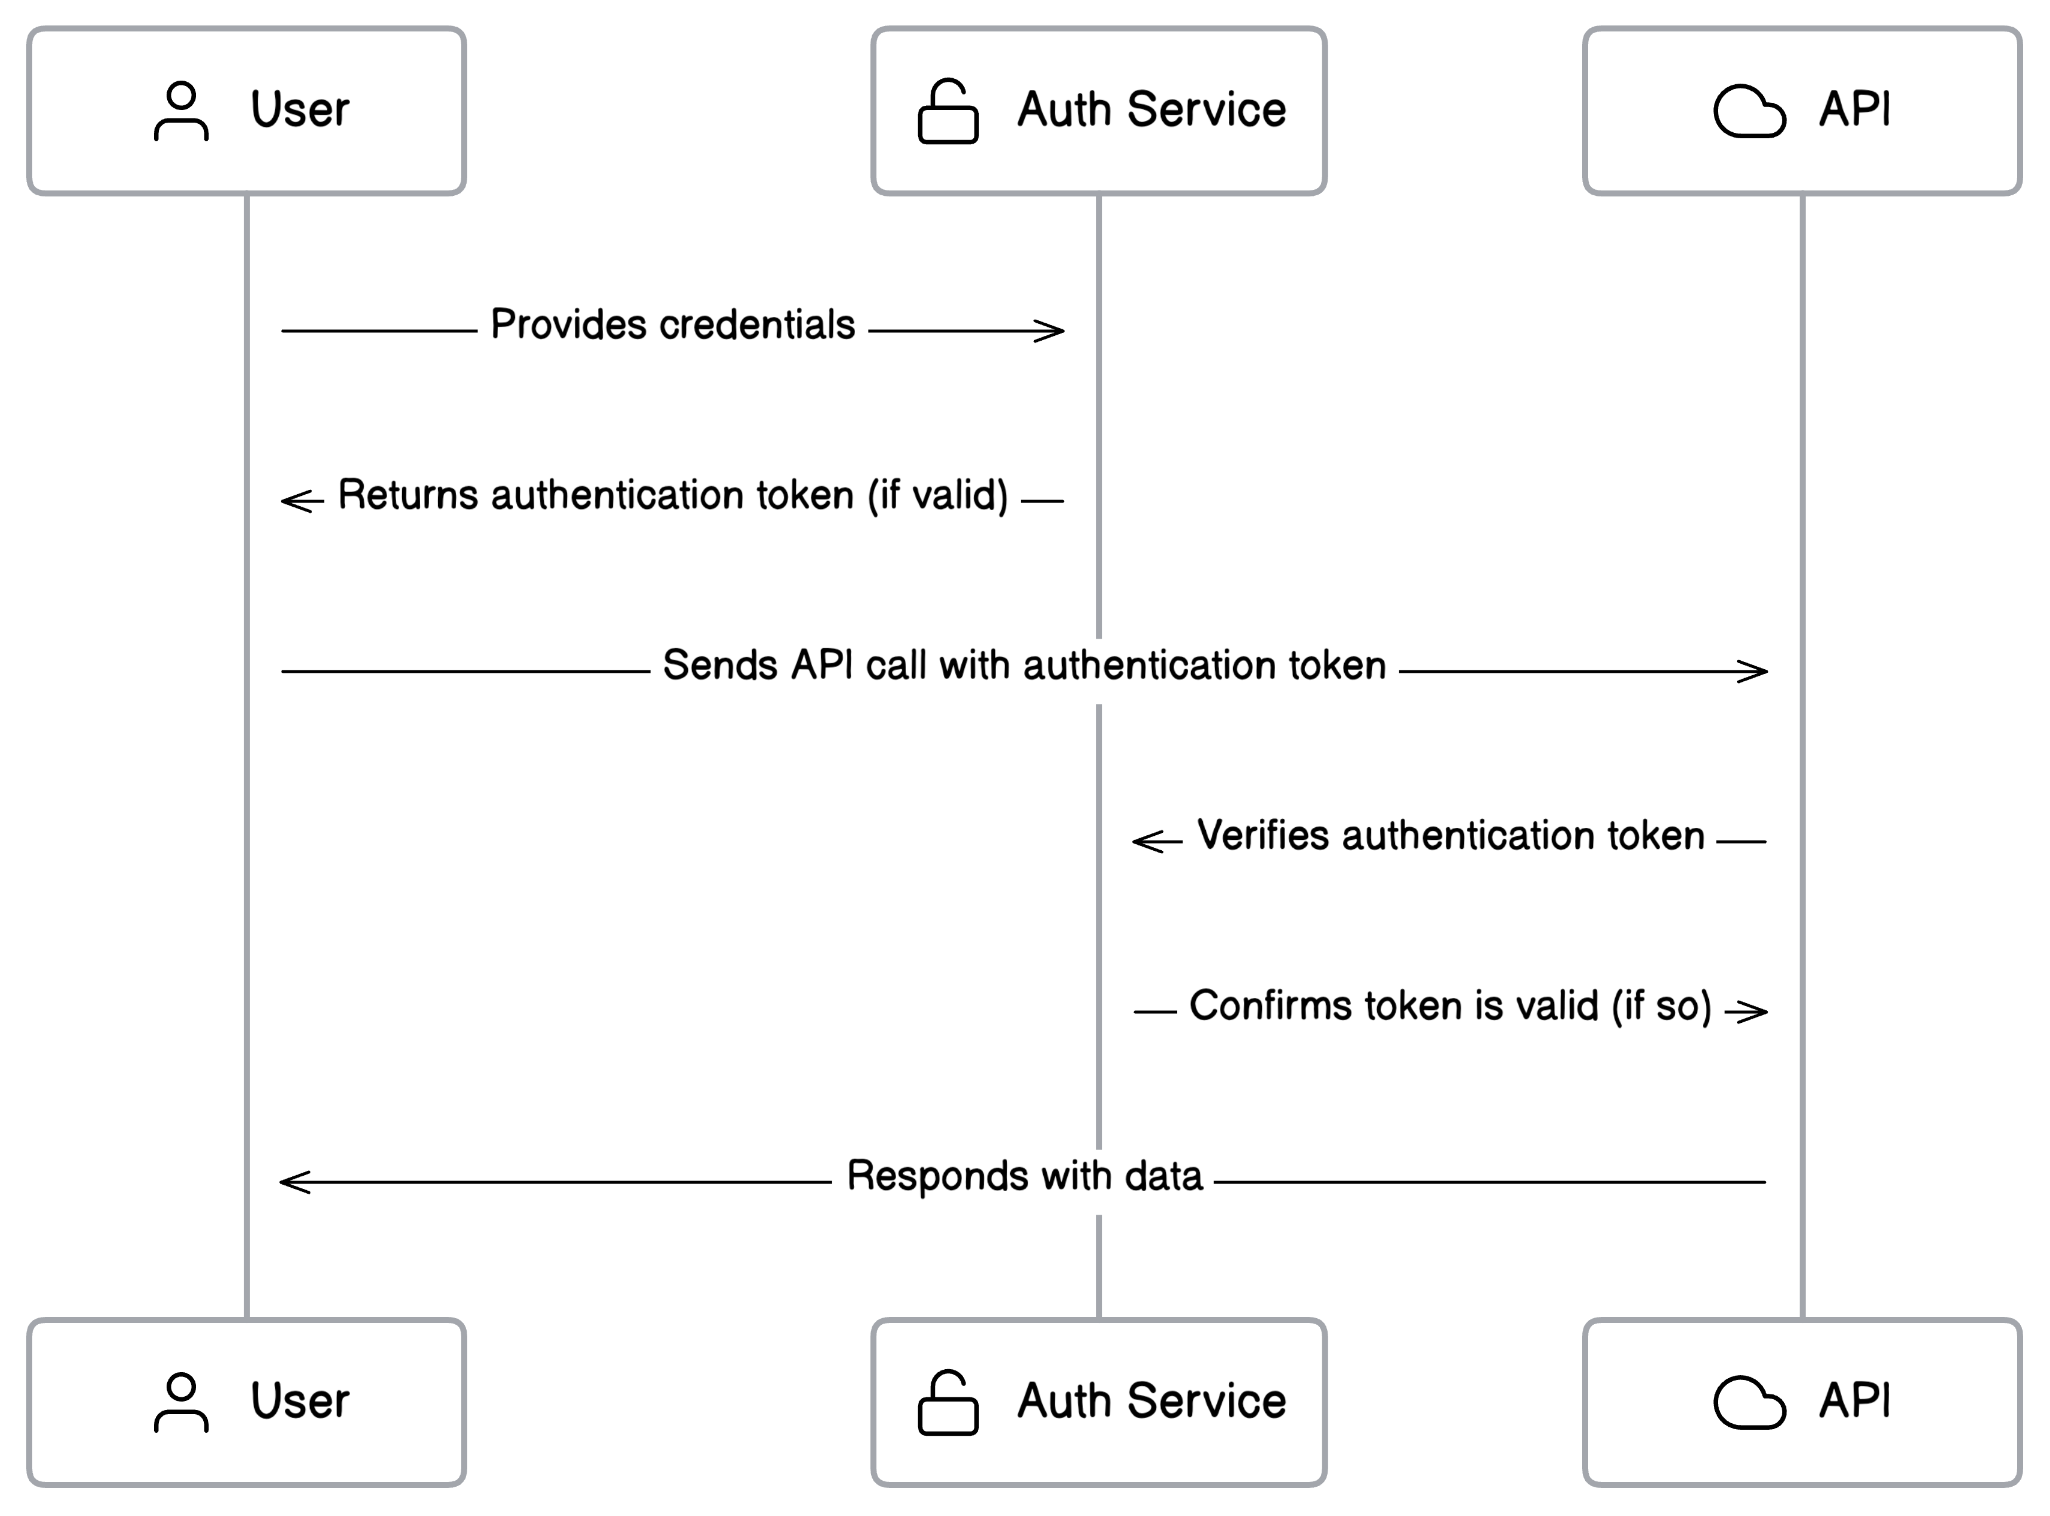
\includegraphics[width=1\textwidth]{pictures/oauth2-diagram.png}
	\caption{Autentizační diagram protokolu OAuth 2.0}
	\label{fig:oauth2Diagram}
\end{figure}


Nejprve se uživatel přihlásí do systému - nejčastěji formou uživatelského jména a hesla, nebo client\_id a client\_secret. Tím pošle HTTP požadavek na endpoint. Autorizace uživateli následně
vrátí token. Pokud má uživatel již platný token, může přistupovat k datům. Naopak pokud mu token již expiroval nebo není platný, volání do API mu vrátí chybové hlášení. 

Součástí autorizační odpovědi bývá i několik dalších údajů. Odpověď může vypadat např. jako na výpisu \ref{tokenResponse}. 

\begin{lstlisting}[language=json, caption={Ukázková odpověď autorizačního serveru}, label=tokenResponse]
{
	"access_token": "ABCDEF1234567890GHIJKL",
	"token_type": "Bearer",
	"expires_in": 3600,
	"refresh_token": "ZYXWVU0987654321DCBANMLKJIHGFEDCBA",
	"scope": "create"
}
\end{lstlisting}
	  
Odpověď bývá ve formátu JSON a obsahuje informace o daném tokenu. Kromě přístupového tokenu obsahuje i refresh\_token, který slouží k obnově tokenu po vypršení jeho platnosti (expires\_in - platnost je v sekundách). To umožňuje uživateli 
používat stále jeden token bez nutnosti generování nového. Dále obsahuje atribut scope, který specifikuje práva uživatele a atribut token\_type \cite{oauthResponseExample}.

%
% Podkapitola existující řešení
%
\section{Existující řešení}
Embedded analytics problematikou se zabývá mnoho firem a každá z nich disponuje jinými způsoby řešení. Zde budou zmíněny firmy, které se objevují často na vrchních příčkách
internetových recenzí či firmy, které byly pro inspiraci doporučeny externím zadavatelem. Pro aktuálnost jsou brány informace ze zdrojů z roků 2022/2023.

Firma GoodData byla zmíněna zadavatelem jako jedna z nejvýraznějších na trhu. Dodává embedded analytics systémy firmám jako je VISA, Zalando či Bentley \cite{goodDataEmbeddingPlatform}. 
Embedování provádí třemi zmíněnými způsoby - HTML iFramem, webovou komponentou či React SDK. Zákazníkům nabízí přizpůsobení dashboardů tak, aby odpovídaly zákazníkovo značce. GoodData získaly
v roce 2023 hned několik ocenění firmou TrustRadius, důvěryhodnou platformou v oblasti B2B (bussines to bussines) \cite{trustRadiusDiscusionGoodData}. Firma GoodData obdržela ocenění Best Value for Price,
Best Relationship či Top Rated 2023. Recenze zákazníků firmy GoodData si chválí hlavně snadné používání, zákaznickou podporu, širokou škálu podporovaných databází či uživatelsky přívětivé
rozhraní \cite{trustRadiusDiscusionGoodData}. Naopak se zmiňují, že dokumentace může být nedostačující či některé endpointy v API mají neintuitivní parametry. I tak ale 92\% recenzentů uvádí,
že by si produkt zakoupili znovu.

Mezi často zmiňovaným produktem je Microsoft Power BI, který je ve svém oboru nejlepší v oblasti bezpečnosti a zabezpečení \cite{bestEmbTools2023},
jelikož Microsoft zaměstnává více než 3500 bezpečnostních expertů. V produktu nabízí také tzv. playground, který
umožňuje uživatelům testovat funkce a vlastnosti daných dashboardů před úplným nasazením. Je také podporvána integrace s cloudovou službou Microsoft Azure. Na webu TrustRadius je k 
Microsoft Power BI podstatně méně recenzí než k produktu GoodData (5x méně). Uživatelé zmiňují dlouhou dobu při zpracování většího objemu dat či vysokou provozní cenu \cite{trustRadiusDiscusionAzure}.

V oblasti modelování data vyniká platforma Powered by Looker \cite{bestEmbTools2023}. Jedná se o produkt služby Google Cloud, který poskytuje způsob, jak sledovat změny a prohlížet jejich
historii v databázi. Disponuje modelovacím jazykem LookML založeným na SQL, který slouží k vytváření sémantických datových modelů. Pomocí něj lze popisovat jednotlivé dimenze, agregáty,
výpočty či datové vztahy v databázi \cite{googleLookMLDoc}. Z toho vyplývá, že datové modely jsou rozšiřitelné, opakovatelně použitelné a konzistentní a tudíž efektivní. V roce 2022 byl tento produkt
oceněn Top Rated a Most Loved společností TrustRadius \cite{trustRadiusDiscusionLooker}. Uživatelé zmiňují, že produkt může být pomalejší a že nástroje na přizpůsobení dashboardů by mohly být
vylepšeny a rozšířeny.
% _____________________________________________________________________________
%
%
%        CHAPTER Návrh knihovny
%
% _____________________________________________________________________________
%
\chapter{Návrh knihovny a uživatelského rozhraní}

\section{Technologie}
\subsection{JavaScript a React}
Pro vývoj knihovny bude využit JavaScript s knihovnou React. Důvodem zvolení těchto technologií je požadavek ze strany zadavatele. React a JavaScript jsou dnes
široce používané technologie ve vývoji webových aplikací. 

React je snadný na naučení, obsahuje málo konceptů, které je třeba se naučit \cite{whyUsingReact}. Jeho instalace je snadná -
stačí pouze naimportovat jeho knihovnu. Využívá speciální JSX syntaxe, která sice vypadá jako HTML, ale ve skutečnosti je tato syntaxe převáděna na HTML. Jelikož je React hojně využíván
v Facebook aplikaci či na Instagramu, dostává se mu velké podpory právě i z tohoto odvětví - čtyři největší přispěvatelé knihovny React jsou zaměstnanci Facebooku \cite{whyUsingReact}. Kromě 
Facebooku využívají React značky jako jsou např. Netflix, airbnb, BBC News či PayPal \cite{whyUsingReact2}. Díky virtualizaci a uchováváním DOM poskytuje React
velmi rychlé vykreslování, přičemž všechny změny se snadno promítají do virtuálního DOM.

DOM (Document Object Model) je strukturovaná reprezentace jazykla HTML, které reprezentuje celé uživatelské rozhraní jakos stromovou datovou strukturu \cite{whatIsDOM}. Každý prvek uživatelského
rozhraní tvoří v DOM stromu právě jeden uzel. Dojde-li ke změně uživatelského rozhraní, DOM se aktualizuje 	a při každé změně se vykresluje znovu, což výrazně ovlivňuje výkon aplikace. 
Toto lze vyřešit použitím virtuálního DOM. Při přidávání nových věcí do aplikace se vytvoří virtuální DOM, která je reprezentován jako strom. Novější virtuální DOM se porovnává se starším, aby
zaznamenal změny. Poté zjistí, jak je možné tyto změny provést pomocí skutečného DOM a aktualizované prvky se následně vykreslí.

Na popularitě Reactu přidává také použití knihovny Redux, která umožňuje uchování dat jako jeden objekt (stav). K tomuto objektu se dá pak jednoduše přistupovat, což značně usnadňuje práci s daty.
Je-li tento stav změněn, aplikace se překreslí a zobrazení se stále synchronizuje se souvisejícími daty \cite{whyUsingReact2}. 

React se kvůli těmto vlastnostem doporučuje využívat u:
\begin{enumerate}
\item Obsáhlých uživatelských rozhraní
\item Rozsáhlých aplikací
\item Aplikací náročné na výkon
\item Multi-platformních aplikací
\end{enumerate}

\subsection{API}	
Data, která budou následně vizualizována knihovnou, budou získávána prostřednictvím Emplifi Public API. Toto rozhraní poskytuje klientům snadný a oblíbený způsob, jak získat přístup k potřebným datům. 
\subsection{OAuth 2.0}
Přístup k datům bude zabezpečen protokolem OAuth 2.0. To umožní nejen autentizaci uživatele, ale také umožné uživatelům udělovat patřičná omezení (např. které endpointy může běžný uživatel volat).

\section{Funkcionality}
\subsection{Komunikace s API}
Navrhovaná knihovna bude vybavená funkcionalitou pro provádění dotazů na Emplifi Public API, což umožní získávat potřebná data pro vizualizaci.
Bude také umět reagovat na chybové odpovědi ze strany API (např. nevalidní token, špatný request, neexistující data apod.). 
\subsection{Playground}
Vytvoření playgroundu umožní uživatelům náhled na vizualizace, které budou chtít embedovat v aplikacích třetích stran. To se může využít zejména pokud si budou chtít ověřit funkčnost či pozměnit
design vizualizace. 
\subsection{Obnova OAuth 2.0 tokenů}
K dispozici bude uživatelské rozhraní, které umožní snadné vytvoření či obnovení OAuth 2.0 tokenu. Jedná se o důležitou funkcionalitu, aby budoucí uživatelé nemuseli složitě získávat
token, ale stačilo jim k tomu pouze jednoduché rozhraní. 
\subsection{PreJSON}
Interní knihovna, která bude zveřejněna během příštího roku. Informace budou dopsány, jakmile bude zveřejněna (včetně vhodné ukázky). Slouží k tomu, aby se do schémat grafů daly jednoduše
vkládat hodnoty. Např. zavoláním Emplifi Public API se vrátí schéma grafu, které bude ukazovat aktivitu uživatelů za posledních X dní. Díky PreJSON knihovně se mohou jednoduše do tohoto schématu
vkládat hodnoty, na kterých je graf závislý (v tomto případě počet dní). Bude poskytnuta i dokumentace, až se tato knihovna zveřejní, takže poté odcituju a provede ukázku.


% _____________________________________________________________________________
%
%
%        CHAPTER Závěr
%
% _____________________________________________________________________________
%
\chapter{Závěr}
Aktuálně je praktická část bakalářské práce ve formě, kdy React aplikace dokáže vizualizovat grafy. Grafy lze vizualizovat pomocí playgroundu, kterému bude v budoucnu ještě upraven
frontend. Zároveň aplikace dokáže obnovovat OAuth2 tokeny (jak token pro Emplifi Public Api, který vrací schémata widgetů, tak i token pro Omni Api, který vrací data do widgetů). Toto je
udělané pouze formou dvou tlačítek. Ty jsou automaticky vypnuté, pokud jsou tokeny validní - momentálně se uchovávají v local storage webového prohlížeče. Externí zadavatel určí co dále. 
Jsou i vypisovány základní stavy tokenu (platný, neplatný, neexistující) a vizualizace v playground nelze embedovat, dokud tyto tokeny nejsou platné. Playground umožňuje uživatelům widgety
i upravovat - například zadáním CSS stylu či zadáním šířky/výšky. Pro debuggování a kontrolu jsou umožněny i výpisy schémat daného widgetu - ty se ovládají jednoduchým přepínačem. Jsou 
ošetřeny základní chyby, které mohou nastat při vizualizaci (chybějící tokeny, nezadané parametry pro PreJSON apod.). 

Nyní bych rád pokračoval v zefektivnění kódu, dopsáním dokumentačních komentářů, napsáním jednotkových testů pro kritické sekce programu, zlepšení frontendu pro playground a pro rozhraní pro
obnovu OAuth 2.0 tokenů. Zároveň bude třeba ošetřit všechny výjimky, které mohou nastat. Dalším krokem bude převést React aplikaci na knihovnu a domluvit se se zadavatelem, jak pokračovat dále -
například zda-li stačí vizualizovat jednotlivé widgety, nebo celé dashboardy. Jako poslední budou provedeny i funkcionální testy podle scénářů, které budou přiloženy ve finálním odevzdání bakalářské práce.

\appendix
\backmatter
\printbibliography
\listoffigures
\listoftables
\listoflistings
% _____________________________________________________________________________
%
%		BACK COVER
% _____________________________________________________________________________
%
\setbackpageqrcode
\backpage
\end{document}